\documentclass{standalone}
\usepackage{pst-eucl}
\usepackage{tikz}
\usepackage{pgfplots}
\usepackage{graphicx}
\usepackage{caption}
\usepackage{subcaption}
\usepackage{stfloats}



%\usepackage{flushend}

%\usepackage[style=ieee]{biblatex}

%\bibliography{EMS2013_KieslichC}

\usetikzlibrary{intersections,positioning,calc,patterns}



\tikzsetnextfilename{importantFigure}
\usepackage{tikz}
% all other packages and stuff you need for the picture
%
\begin{document}
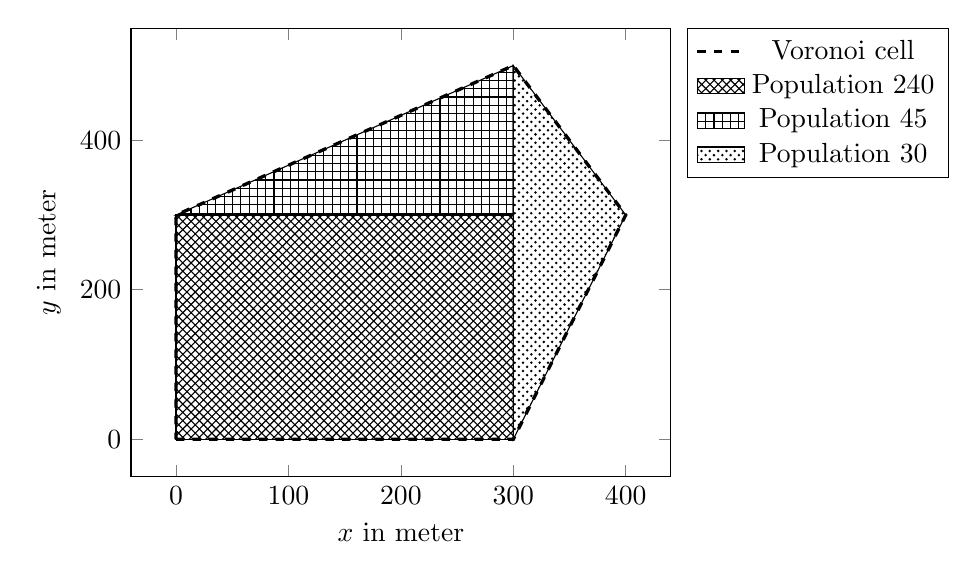
\begin{tikzpicture}s
    \begin{axis}[
        xlabel=$x$ in meter,
        ylabel=$y$ in meter,
        legend pos=outer north east]
   
    \addplot+[mark=none,draw=black, very thick,dashed] coordinates 
		{(0,0) (300,0) (400,300) (300,500) (0,300)} -- cycle;
    \addlegendentry{Voronoi cell} 
    
     \addplot+[mark=none,pattern=crosshatch,area legend,draw=black] coordinates 
		{(0,0) (300,0) (300,300) (0,300)} -- cycle;
    	\addlegendentry{Population 240}
    	
    	\addplot+[mark=none,pattern=grid,area legend,draw=black] coordinates 
		{(0,300) (300,300) (300,500) (0,300) } -- cycle;
    	\addlegendentry{Population 45}
    	
    	\addplot+[mark=none,pattern=crosshatch dots,area legend,draw=black] coordinates 
		{(300,0) (300,500) (400,300) }-- cycle;
    	\addlegendentry{Population 30}
    
	     
    
    \end{axis}
\end{tikzpicture}
\end{document}

